
%%%%%%%%%%%%%%%%%%%%%%%%%%%%%%%%%%%%%%%%%%%%
% POLICY
%%%%%%%%%%%%%%%%%%%%%%%%%%%%%%%%%%%%%%%%%%%%

\chapter{Policy}

A reinforcement learning system consists of four main elements:
\begin{itemize}
%\setlength{\itemsep}{0pt}
%\setlength{\parsep}{0pt}
\setlength{\parskip}{0pt}
\item[1.]
An agent
\item[2.]
A policy 
\item[3.]
A reward signal, and 
\item[4.]
A value function
\end{itemize}

An agent's behaviour at any point of time is defined in terms 
of a policy. A {\bf policy} is like a blueprint of the connections 
between perception and action in an environment.  

In the first section, we introduce what is a policy.
Later in the second section we talk about policy types.
In the third section, we shall discuss the key differences 
in the two main kind of policies: 
\begin{itemize}
\item On-policy reinforcement learning
\item Off-policy reinforcement learning
\end{itemize}

\section{What is a Policy}

In this section, we'll study the concept of policy for 
reinforcement learning\cite{Gabriele2020}
\parencite{Gabriele2020}
.

At the end of this section, we'll be familiar with the basic 
notions of reinforcement learning and its policy-based methods.

\subsection{The Definition of a Policy}

Reinforcement learning is a branch of machine learning 
dedicated to training agents to operate in an environment, 
in order to maximize their utility in the pursuit of some 
goals.

Its underlying idea is that intelligence is an emergent 
property of the interaction between an agent and its 
environment. This property guides the agent's actions by 
orienting its choices in the conduct of some tasks.

We can say, analogously, that intelligence is the capacity 
of the agent to select the appropriate strategy in relation 
to its goals. Strategy, a teleologically-oriented subset of 
all possible behaviors, is here connected to the idea of 
"policy".

{\bf A policy is, therefore, a strategy that an agent uses 
in pursuit of goals}. The policy dictates the actions that 
the agent takes as a function of the agent's state and the 
environment.

\subsection{Mathematical Definition of a Policy}

With formal terminology, we define a policy $\pi$ in terms 
of the {\bf Markov Decision Process} to which it refers. 
A Markov Decision Process is a tuple of the form 
$(S, A, P, R)$, structured as follows.

The first element is a set $S$ containing the internal 
states of the agent. Together, all possible states span a 
so-called state space for the agent. In the case of the grid 
worlds for agent simulations, $S$ normally consists of the 
position of the agent on a board plus, if necessary, some 
parameters.

The second element is a set $A$ containing the actions of 
the agent. The actions correspond to the possible behaviors 
that the agent can take in relation to the environment. 
Together, the set of all actions spans the action space for 
that agent.

An action can also lead to a modification of the state of 
the agent. This is represented by the matrix $P$ containing 
the probability of transition from one state to another. 
Its elements, $P_a(s,s')$, contain the probabilities 
$Pr(s' | s, a)$ for all possible actions $a\in A$ and pairs 
of states $(s, s')$.

The fourth element $R(s)$ comprises the reward function for 
the agent. It takes as input the state of the agent and 
outputs a real number that corresponds to the agent's reward.

We can now formally define the policy, which we indicate with 
$\pi(s)$. {\bf A policy $\pi(s)$ comprises the suggested 
actions that the agent should take for every possible 
state $s\in S$}.

\subsection{策略需要有探索能力(随机性)}

抛开RL算法的细节,几乎所有RL算法可以抽象成如下的形式:
\begin{figure}[ht]
\centering
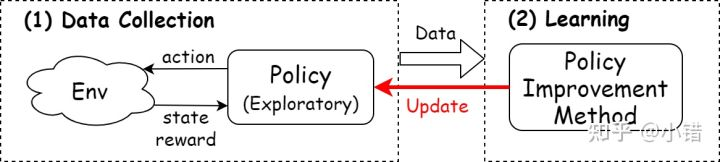
\includegraphics[scale=0.5]{pix/exploration.jpg}
\caption{Two tasks of an RL algorithm}
%\label{fig:label}
\end{figure}

RL 算法中都需要做两件事:
\begin{itemize}
%\setlength{\itemsep}{0pt}
%\setlength{\parsep}{0pt}
\setlength{\parskip}{0pt}
\item[(1)]
收集数据(Data Collection):与环境交互,收集学习样本; 
\item[(2)]
学习(Learning)样本:学习收集到的样本中的信息,提升策略。
\end{itemize}

RL 算法的最终目标是学习每种状态下最优的动作,而在训练过程中,
收敛(到最优策略 $\pi^*$)前的当前策略 $\pi$ 并非最优,所以它提供的动作并非最优。
为了找到动作空间里潜在的最优动作,算法必须尝试当前策略 $\pi$ 认为的非最优的动作,
因此 RL 算法中的策略需要有随机探索(Exploration)的能力。

\subsection{策略如何做到随机探索}

RL算法中的策略分为确定性(Deterministic)策略与随机性(Stochastic)策略:
\begin{itemize}
%\setlength{\itemsep}{0pt}
%\setlength{\parsep}{0pt}
\setlength{\parskip}{0pt}
\item
确定性策略 $\pi(s)$ 为一个将状态空间 $S$ 映射到动作空间 $A$ 的函数,即 
$\pi : S \rightarrow A$。它本身没有随机性质,因此通常会结合 $\epsilon-\text{greedy}$ 
或往动作值中加入高斯噪声的方法来增加策略的随机性。
\item
随机性策略 $\pi(A_t | S_t)$ 是条件为 $S_t \in S$ 情况下,动作 $A_t$ 的条件概率分布。
它本身带有随机性,获取动作时只需对概率分布进行采样即可。
\end{itemize}

为了不让思路凌乱,这里仅讨论 $Q$ 函数构造的确定性策略及其增加随机性的方式。
用 $Q$ 函数构造确定性策略是一种常见的策略形式,其具体方式是:
$$
\pi(s)= \arg \underset{a}{\max}\; Q(s, a)
$$

即选取 $Q$ 值最大的动作为最优动作。(注意:一般只有在动作空间离散的情况下采用这种策略,
若动作空间连续上式中的最大化操作需要经过复杂的优化求解过程。)

可用 $\epsilon-\text{greedy}$ 方法将上述确定性策略改造成具有探索能力的策略:
$$
\pi_\epsilon(s)=\begin{cases}
\arg\max_a\; Q(s,a), &\text{with probability } 1 - \epsilon \\
\text{random action}, &\text{with probability } \epsilon
\end{cases}
$$

即,以 $\epsilon$ 的概率选择随机动作(Exploration),以 $1 - \epsilon$ 
的概率按照确定性策略 $\pi(s)$ 选取动作。


\subsection{Example of a Policy}

Let's now see an example of policy in a practical scenario, 
to better understand how it works. In this example, an agent 
has to forage food from the environment in order to satisfy 
its hunger. It then receives rewards on the basis of the 
fruit it eats:

\begin{figure}[ht]

\centering
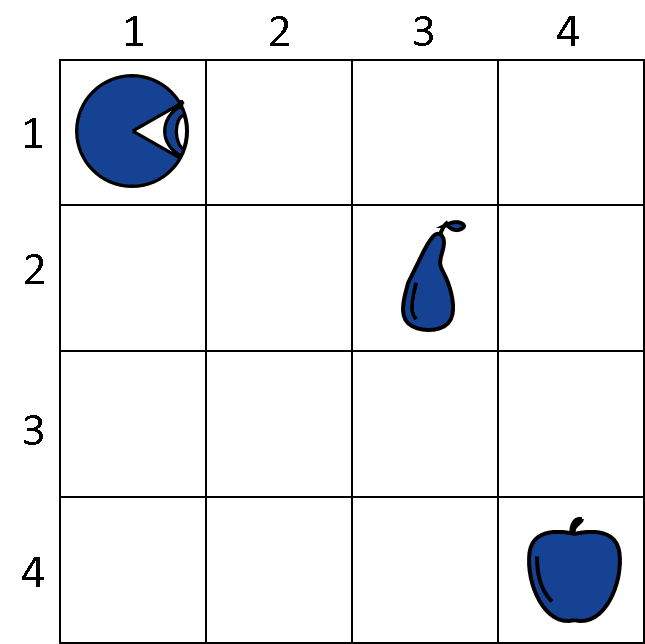
\includegraphics[scale=0.5]{pix/example1.png}
\caption{example figure}
%\label{fig:label}
\end{figure}

The internal state of the agent corresponds to its location 
on the board, in this case, $s_t = (x,y)$ and $s_0 = (1,1)$. 
The action space, in this example, consists of four possible 
behaviors: $A = \text{up, down, left, right}$. The probability 
matrix $P$ contains all pairwise combinations of states 
$(s, s')$ for all actions in $A$. It's Bernoulli-distributed, 
and looks like this:
\begin{align*}
P_{\text{down}}( (1,1), (1,2) ) &= 1; \\
P_{\text{down}}( (1,1), (1,3) ) &= 0; \\
... ; \\
P_{\text{up}}( (4,4), (4,3) ) &= 1
\end{align}

The reward function $R$ is defined in this manner. If it's 
in an empty cell, the agent receives a negative reward of 
$-1$, to simulate the effect of hunger. If instead, the 
agent is in a cell with fruit, in this case, $(3,2)$ for 
the pear and $(4,4)$ for the apple, it then receives a 
reward of $+5$ and $+10$, respectively.

The reward function $R$ thus looks like this:
\begin{align*}
R(\text{No fruit}) &= -1 \\
R(\text{Pear}) &= +5 \\
R(\text{Apple}) &= +10
\end{align}

The simulation runs for an arbitrary finite number of time 
steps but terminates early if the agent reaches any fruit.



\subsection{Evaluation of the Policies}

The agent then considers two policies $\pi_1$ and $\pi_2$. 
If we simplify slightly the notation, we can indicate a 
policy as a sequence of actions starting from the state of 
the agent at $s_0$:

\begin{itemize}
%\setlength{\itemsep}{0pt}
%\setlength{\parsep}{0pt}
\setlength{\parskip}{0pt}
\item[1.]
$\pi_1 = \text{down, right, right} \to \text{Pear}$

\item[2.]
$\pi_2 = \text{right, right, right, down, down, down} \to \text{Apple}$

\end{itemize}


\begin{figure}[ht]
\centering
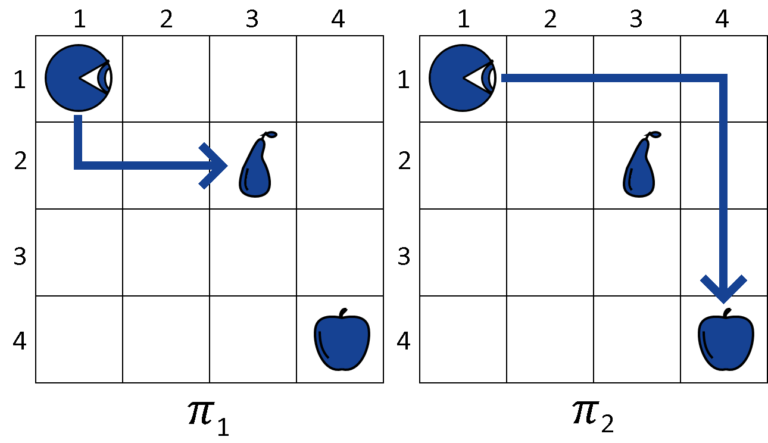
\includegraphics[scale=0.3]{pix/example1_1.png}
\caption{example figure1}
%\label{fig:label}
\end{figure}

The agent then has to select between the two policies. 
By computing the utility function $U$ over them, the 
agent obtains:

\begin{align*}
U(\pi_1) &= -1-1+5 = +3 \\
U(\pi_2) &= -1-1-1-1-1+10 = +5
\end{align}

\begin{figure}[ht]

\centering
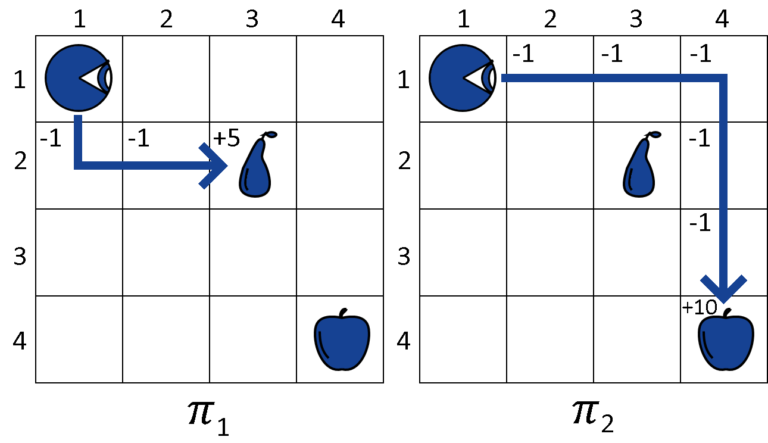
\includegraphics[scale=0.3]{pix/example1_2.png}
\caption{example figure2}
%\label{fig:label}
\end{figure}

The evaluation of the policies suggests that the utility 
is maximized with $\pi_2$, which then the agent chooses 
as its policy for this task.


%+++++++++++++++++++++++++++++++++++++++++++
% Policy Types
%-------------------------------------------

\section{Policy Types}

{\bf Deterministic and Stochastic Policies Explained} \cite{Loevenich2021}

行为策略是用来与环境互动产生数据的策略,即在训练过程中做决策;而目标策略在行为策略产生的
数据中不断学习、优化,即学习训练完毕后拿去应用的策略。百官(锦衣卫)就是行为策略,
去收集情况或情报,给皇帝(目标策略)做参考来学习,当皇帝收集到的情报越多,能做的决策就越优。

为了解决强化学习问题中的exploitation(利用) 和 exploration (探索),我们可以利用一个
策略(行为策略)来保持探索性,提供多样化的数据,而不断地优化另一个策略(目标策略)。
On-policy 的目标策略和行为策略是同一个策略,其好处就是简单粗暴,直接利用数据就可以优化
其策略,但这样的处理会导致策略其实是在学习一个局部最优,因为On-policy的策略没办法很好的
同时保持既探索又利用;而Off-policy将目标策略和行为策略分开,可以在保持探索的同时,更能求
到全局最优值。但其难点在于:{\bf 如何在一个策略下产生的数据来优化另外一个策略?}

From the previous section we know that a policy is a description of how an 
agent behaves given its current state and the goal. In this section, 
we will discuss Policy Types: Deterministic Policies and Stochastic Policies.

{\bf Deterministic Policies:} In a deterministic policy, the action taken 
at each state is always the same. This can be implemented using a lookup 
table or decision tree. In this case, we denote it is denoted by $\mu$:
$$
a_t = \mu(s_t)
$$

{\bf Stochastic Policies:} A stochastic policy, on the other hand, produces 
different actions from one instance to the next, but these are still chosen 
according to some fixed probabilities. The stochastic policy is denoted by 
$\pi$:
$$
a_t \sim \pi(\cdot | s_t)
$$

Because the policy is essentially the agent's brain, it's not unusual to 
replace "policy" with "agent," such as when someone says, "The agent is 
attempting to maximize reward."

In deep RL, we deal with parameterized policies: policies that produce 
computable functions that are dependent on a set of parameters (for example, 
the weights and biases of a neural network) that may be adjusted to modify 
the outcome using some optimization algorithm. 

Categorical and diagonal Gaussian policies are the two most frequent types 
of stochastic policies in deep RL. Categorical policies can be applied in 
discrete action regions, while diagonal Gaussian policies are appropriate for 
continuous action regions. 

{\bf Categorical Policy:} A categorical policy is a stochastic policy that 
favors either one or zero actions in each state, with equal probabilities 
assigned to all possible action choices.

{\bf Diagonal Gaussian Policy:} On the other hand, Diagonal Gaussian policies 
take any number of actions from zero to infinity and distribute them according 
to a diagonal Gaussian distribution. This means that in any given state, the 
agent can select from many different actions with equal probabilities assigned 
to all possible action choices.

The two most important computations for employing and training stochastic 
policies are:

\begin{itemize}
%\setlength{\itemsep}{0pt}
%\setlength{\parsep}{0pt}
\setlength{\parskip}{0pt}
\item[1)]
Sampling actions from the policy,

\item[2)]
Comparing log-likelihoods of various actions.
\end{itemize}

We'll go through how to implement these for both categorical and diagonal 
Gaussian policies in the following. 



%+++++++++++++++++++++++++++++++++++++++++++
% On-Policy vs Off-Policy
%-------------------------------------------

\section{On-Policy VS Off-Policy}

\cite{Sagar2020}

古时候,优秀的皇帝都秉持着“水能载舟 亦能覆舟”的思想,希望能多了解民间百姓的生活。
皇帝可以选择通过微服出巡,亲自下凡了解百姓生活(On-policy)。虽然眼见为实,
但毕竟皇帝本人分身乏术,掌握情况不全;因此也可以派多个官员去了解情况,
而皇帝本人则躺在酒池肉林里收听百官情报即可(Off-policy)。

Comparing reinforcement learning models for hyperparameter optimization is 
an expensive affair, and often practically infeasible. So the performance of 
these algorithms is evaluated via on-policy interactions with the target 
environment. These interactions of an on-policy learner help get insights 
about the kind of policy that the agent is implementing.

An off-policy, whereas, is independent of the agent's actions. It figures 
out the optimal policy regardless of the agent's motivation. For example, 
Q-learning is an off-policy learner.

On-policy methods attempt to evaluate or improve the policy that is used to 
make decisions. In contrast, off-policy methods evaluate or improve a policy 
different from that used to generate the data.

Here is a snippet from Richard Sutton's book on reinforcement learning where 
he discusses the off-policy and on-policy with regard to Q-learning and 
SARSA respectively:

\subsection{Off-policy}

In Q-Learning, the agent learns optimal policy with the help of a greedy 
policy and behaves using policies of other agents. Q-learning is called 
off-policy because the updated policy is different from the behavior policy, 
so Q-Learning is off-policy. In other words, it estimates the reward for 
future actions and appends a value to the new state without actually following 
any greedy policy.

\subsubsection{Off-policy 将收集数据当做一个单独的任务}

RL 算法中需要带有随机性的策略对环境进行探索获取学习样本,一种视角是:off-policy 
的方法将收集数据作为 RL 算法中单独的一个任务,它准备两个策略:behavior policy and
target policy。行为策略是专门负责学习数据的获取,具有一定的随机性,
总是有一定的概率选出潜在的最优动作。
而目标策略借助行为策略收集到的样本以及策略提升方法提升自身性能,并最终成为最优策略。
Off-policy 是一种灵活的方式,如果能找到一个“聪明的”行为策略,总是能为算法提供最合适的样本,
那么算法的效率将会得到提升。

the learning is from the data off the target policy(引自《Reinforcement 
Learning An Introduction》)。也就是说 RL 算法中,数据来源于一个单独的用于探索的策略
(不是最终要求的策略)。以 Q-Learning 为例,它的算法流程如下:

\begin{figure}[ht]
\centering
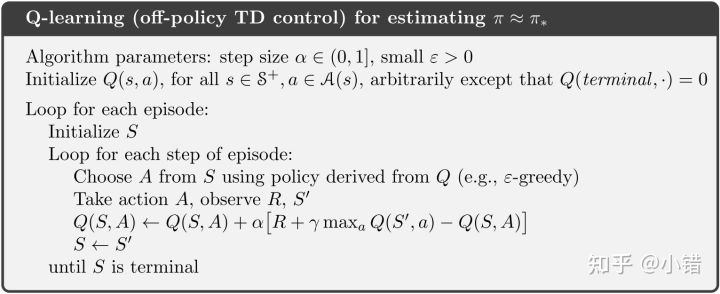
\includegraphics[scale=0.5]{pix/qlearning.jpg}
\caption{Q-Learning}
%\label{fig:label}
\end{figure}

算法流程图不够直观,将算法中的值函数更新式改写成另外一种形式后将算法用图描绘。

\begin{figure}[ht]
\centering
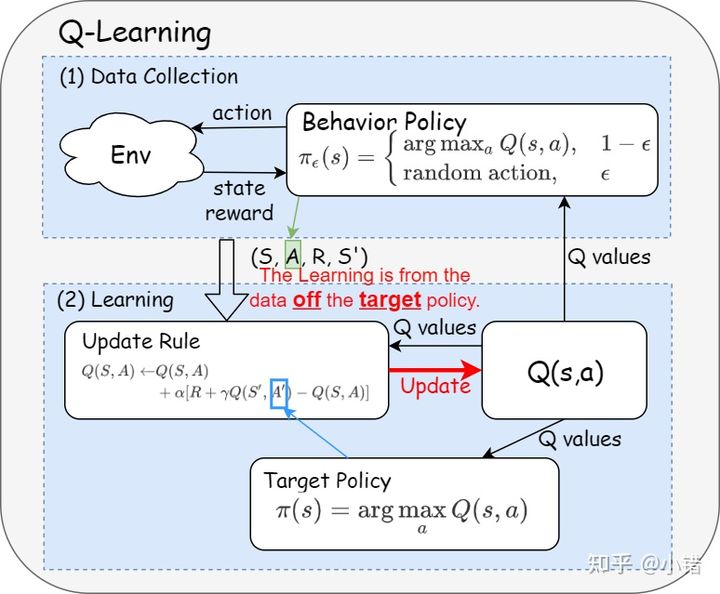
\includegraphics[scale=0.5]{pix/qlearning_flow.jpg}
\caption{Flow of Q-Learning}
%\label{fig:label}
\end{figure}

如图所示,$Q$-Learning 数据收集部分用的是由$Q$函数构造的
$\epsilon-\text{greedy}$策略 $\pi_\epsilon(s)$ (行为策略),而它的最终目标是
greedy 策略$\pi(s)$(目标策略)。$Q$函数更新规则(update rule)中的训练样本
$(S,\; A,\; R,\; S')$是由行为策略$\pi_\epsilon(s)$(而非目标策略)提供,
因此它是典型的 off-policy 方法。

\subsubsection{为什么有时候off-policy需要与重要性采样配合使用?}

重要性采样是用一个概率分布的样本来估计某个随机变量关于另一个概率分布的期望。

假设已知随机策略$\pi(a | s)$,现在需要估计策略$\pi$对应的状态值
$V^\pi$,但是只能用另一个策略$\pi'(a | s)$获取样本。对于这种需要用另外一个策略
的数据(off-policy)来精确估计状态值的任务,需要用到重要性采样的方法,具体做法是在对应
的样本估计量上乘上一个权重($\pi$与$\pi'$的相对概率),称为重要性采样率。

以off-policy Monte Carlo估计为例,它的步骤为:
\begin{itemize}
%\setlength{\itemsep}{0pt}
%\setlength{\parsep}{0pt}
\setlength{\parskip}{0pt}
\item[(1)]
由$\pi'$与环境交互生成一条样本轨迹:$(s_0,a_0,r_0,s_1,a_1,r_1,\dots,s_T,a_T,r_T)$,
$T(s)$表示轨迹样本中状态为$s$时间点的集合。$|T(s)|$为该集合的元素的总数量。
\item[(2)]
$t$时刻之后的轨迹序列关于$\pi$与$\pi'$的似然分别为
$\prod_{k=t}^T\pi(a_k|s_k)Pr(s_{k+1}|s_k, a_k)$与
$\prod_{k=t}^T\pi'(a_k|s_k)Pr(s_{k+1}|s_k, a_k)$,对应的重要性采样率为:
$$
\rho_t^T=\frac{\prod_{k=t}^T\pi(a_k|s_k)Pr(s_{k+1}|s_k, a_k)}{\prod_{k=t}^T\pi'(a_k|s_k)Pr(s_{k+1}|s_k, a_k)}
=\frac{\prod_{k=t}^T\pi(a_k|s_k)}{\prod_{k=t}^T\pi'(a_k|s_k)}
$$
\item[(3)]
$t$时刻之后的总回报为$G_t=\sum_{k=t}^T\gamma^{k-t}r_k$
\item[(4)]
按照MC方法估计状态s对应的状态值:
$$
V(s)=\frac{\sum_{t\in T}\rho_t^TG_t}{|T(s)|}
$$
\end{itemize}
最后再次强调,如果需要用off-policy方法估计/预测状态值或动作值时,需要用到重要性采样。

\subsubsection{为什么Q-Learning算法(或DQN)身为off-policy可以不用重要性采样?}

$Q^*(s,a)$ 为最优策略对应的$Q$函数,最优$Q$函数遵循如下最优贝尔曼等式:
$$
Q^*(s,a)=\sum_{s',r}Pr(s', r | s, a) [r + \gamma \max_{a'}Q^*(s', a')]
$$
{\bf $Q$-Learning的思想是从任意初始化的Q函数出发,以最优贝尔曼方程为标准调整$Q$函数。}
观察$Q$函数在第$n$轮更新时的更新式:
$$
Q_{n+1}(s, a) \leftarrow Q_n(s, a) + \alpha [r + \gamma \max_{a'}Q_n(s', a')
- Q_n(s, a)]
$$
可以看到它实际是以最优贝尔曼的估计量$r + \gamma\, \underset{a'}{\max}Q_n(s', a')$为目标(target),
让$Q_{n+1}(s, a)$尽量靠近该目标。需要注意到:{\bf 最优贝尔曼等式右侧的期望只与状态转移
分布有关而与策略无关,不论训练数据$(S,\; A,\; R,\; S')$来自于哪个策略,按照$Q$-Learning
的更新式更新都能使$Q$函数接近$Q^*(s,a)$。}因此,$Q$-Learning可以不采用重要性采样。
(DQN算法同理)

\subsubsection{重要性采样的数学说明}

为了能从行为策略$b$产生的样本回合(Episode)中评估(学习)策略$\pi$,我们要求当执行
$b$策略时,$\pi$中的每个动作都有一定概率发生,也就是$\pi(a|s)>0$时,必有
$b(a|s)>0$(逆命题不一定成立)。这种要求称为“包含”(Coverage)。在求最优策略的过程中,
目标策略$\pi$通常都是基于当前评估的价值函数$V$的贪婪策略(策略$\pi$的函数$V$的学习数据
来源于策略$b$,但并非直接利用$b$的$V$函数,后面会详细解释)。因此目标策略最终能收敛为
最优策略,而行为策略$b$则保持随机因而具有探索性。

几乎所有的off-policy都利用到一种技巧“Important Sampling”,这种技巧可以解决:
求解一个概率分布(Distribution)的期望值(Expect)时,用来求解该期望值的样本数据是由
另一个概率分布所产生。具体做法是:根据目标策略$\pi$和行为策略$b$分别所产生的相同某段序列
(这里我们把Episode中某一段称为Trajectory)的概率的比值来加权求和return(Return是MC
法中的一个样本序列(整个Episode)的总奖励),这个比值称为{\bf importance-sampling 
ratio}。(也就是把一段又一段的序列总价值根据importance-sampling ratio加权求和,
得到某个state的价值期望)
\begin{equation}\label{sate_gain_expectation}
\rho_t^{T-1}=\frac{\prod_{k=t}^{T-1}\pi(A_k|A_k)p(S_{k+1}|S_k, A_k)}{\prod_{k=t}^{T-1}b(A_k|A_k)p(S_{k+1}|S_k, A_k)}
=\frac{\prod_{k=t}^{T-1}\pi(A_k|S_k)}{\prod_{k=t}^{T-1}b(A_k|S_k)}
\end{equation}

【注意,上式只有当两个策略产生的由$t$到$T-1$的序列完全一样时,才能消掉转移概率。
(实际上排列顺序不一致但出现的转移情况一致也可以消掉转移概率)】

式中$\pi(A_k|S_k)$为策略$\pi$时的动作概率分布,$b(A_k|S_k)$为策略$b$时的动作概率分布。

虽然一个trajectory的发生可能性与环境的动态(即转移概率$p$)有关,但是通过比值可以消掉环
境的动态因素。因此importance-sampling ratio只由策略$b$、策略$\pi$和相应的序列所决定,
与MDP无关。 

因此,当我们评估(Estimate)在目标策略$\pi$下的奖励期望(Expected Return)时,
不能直接使用来自行为策略$b$产生的样本数据所计算得到的奖励期望$E[G_t|S_t]$,因为这样将不能
对样本数据进行平均求和而得到目标策略的价值函数。

\subsubsection{Thinking in variational method}

\begin{minipage}[t][2.5cm][t]{2em}
测试
\end{minipage}
行为策略似乎是在测试空间做添加噪声的处理,而目标策略似乎是在算子空间做逼近处理。
off-policy与on-policy只是选取了概率统计的方式来进行处理的算法选择而已。
%\begin{minipage}[c][2.5cm][t]{2em}
%测试2
%\end{minipage}

\subsection{On-policy}

SARSA (state-action-reward-state-action) is an on-policy reinforcement 
learning algorithm that estimates the value of the policy being followed. 
In this algorithm, the agent grasps the optimal policy and uses the same to 
act. The policy that is used for updating and the policy used for acting is 
the same, unlike in Q-learning. This is an example of on-policy learning.

An experience in SARSA is of the form $⟨S,A,R,S', A' ⟩$, which means that

\begin{itemize}
%\setlength{\itemsep}{0pt}
%\setlength{\parsep}{0pt}
\setlength{\parskip}{0pt}
\item
current state $S$, 
\item
current action $A$, 
\item
reward $R$, and 
\item
new state $S'$,
\item
future action $A'$. 

\end{itemize}

This provides a new experience to update from
$$
Q(S,A)\quad \text{to}\quad R + \gamma\, Q(S', A').
$$

on-policy的特点就是:the target and the behavior polices are the same。
也就是说on-policy里面只有一种策略,它既为目标策略又为行为策略。SARSA算法即为典型的
on-policy的算法,下图所示为SARSA的算法示意图,可以看出算法中只有一种策略,
训练的数据来自于它。

\begin{figure}[ht]
\centering
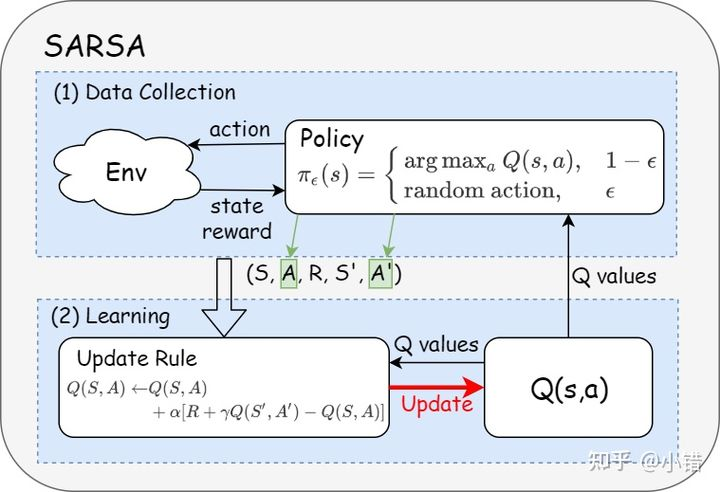
\includegraphics[scale=0.5]{pix/SARSA_flow.jpg}
\caption{Flow of SARSA algorithm}
%\label{fig:label}
\end{figure}

\subsubsection{SARSA算法(on-policy)像是在进行值函数估计,为什么能收敛到最优策略?}

更新式中用到的策略也是$\epsilon$-greedy算法。$\epsilon$的概率是用随机动作,
对策略的提升没有帮助;但另外有$1-\epsilon$的概率,按照
$\arg \underset{a}{\max}\, Q(s,a)$选取动作,即对策略进行提升。{\bf 可以发现
$\epsilon$-greedy策略是一种完全不同于用条件概率分布表示的策略,只要$\epsilon$较小,
它自带策略提升的功能。}


\subsection{Conclusion}

On-policy reinforcement learning is useful when you want to optimize the 
value of an agent that is exploring. For offline learning, where the agent 
does not explore much, off-policy RL may be more appropriate.

For instance, off-policy classification is good at predicting movement in 
robotics. Off-policy learning can be very cost-effective when it comes to 
deployment in real-world, reinforcement learning scenarios. The 
characteristic of the agent to explore and find new ways and cater for the 
future rewards task makes it a suitable candidate for flexible operations. 
Imagine a robotic arm that has been tasked to paint something other than 
what it is trained on. Physical systems need such flexibility to be smart 
and reliable. You do not want to hardcode use cases today. The goal is to 
learn on the go.

However, off-policy frameworks too are not without any disadvantages. 
Evaluation becomes challenging as there is too much exploration. These 
algorithms might assume that an off-policy evaluation method is accurate in 
assessing the performance. But agents fed with past experiences may act very 
differently from newer learned agents, which makes it hard to get good 
estimates of performance. 

Promising directions for future work include developing off-policy methods 
that are not restricted to success or failure of reward tasks, but extending 
the analysis to stochastic tasks as well.

For more information, check Richard Sutton's book.

% https://web.stanford.edu/class/psych209/Readings/SuttonBartoIPRLBook2ndEd.pdf

\begin{itemize}
%\setlength{\itemsep}{0pt}
%\setlength{\parsep}{0pt}
\setlength{\parskip}{0pt}
\item
off-policy的最简单解释: the learning is from the data off the target policy。
\item
On/off-policy的概念帮助区分训练的数据来自于哪里。
\item
Off-policy方法中不一定非要采用重要性采样,要根据实际情况采用(比如,需要精确估计值函数时
需要采用重要性采样;若是用于使值函数靠近最优值函数则不一定)。
\end{itemize}

%.............................
% 2.3.3
\subsection{What is the difference between Q-learning and SARSA?}

https://stackoverflow.com/questions/6848828/what-is-the-difference-between-q-learning-and-sarsa

\subsubsection{提问者自己的作答}

SARSA is on-policy while Q-learning is off-policy, but when looking at their 
formulas it's hard to see any difference between these two algorithms.

According to the book Reinforcement Learning: An Introduction 
(by Sutton and Barto \cite{Sutton1998}). In the SARSA algorithm, given a 
policy, the corresponding action-value function $Q$ (in the state $s$ and action 
$a$, at timestep $t$), i.e. $Q(s_t, a_t)$, can be updated as follows
$$
Q(s_t, a_t) = Q(s_t, a_t) + \alpha *(r_t + \gamma *Q(s_{t+1}, a_{t+1}) - Q(s_t, a_t))
$$
On the other hand, the update step for the Q-learning algorithm is the following
$$
Q(s_t, a_t) = Q(s_t, a_t) + \alpha *(r_t + \gamma *\max_aQ(s_{t+1}, a) - Q(s_t, a_t))
$$
which can also be written as
$$
Q(s_t, a_t) = (1-\alpha)*Q(s_t, a_t) + \alpha * (r_t+\gamma *\max_aQ(s_{t+1}, a))
$$
where $\gamma$ is the discount factor and $r_t$ is the reward received from 
the environment at timestep $t$.

Is the difference between these two algorithms the fact that SARSA only looks 
up the next policy value while Q-learning looks up the next maximum policy value?

The post writer has made a github repo
http://alexge233.github.io/relearn/
playing with Q-learning  and empirically understood what the difference is.
It all amounts to {\bf how you select your next best action}, which from an 
algorithmic standpoint can be a mean, max or best action depending on how 
you chose to implement it.

The other main difference is when this selection is happening (e.g., online 
vs offline) and how/why that affects learning. If you are reading this in 
2019 and are more of a hands-on person, playing with a RL toy problem is 
probably the best way to understand the differences.

One last {\bf important} note is that both Suton & Barto as well as Wikipedia 
often have mixed, confusing or wrong formulaic representations with regards 
to the next state best/max action and reward:
\begin{emp_box}
$r(t+1)$
\end{emp_box}
is in fact
\begin{emp_box}
$r(t)$
\end{emp_box}
Hope this helps anyone ever getting stuck at this.

\subsubsection{Another answer}

When I was learning this part, I found it very confusing too, so I put 
together the two pseudo-codes from R.Sutton and A.G.Barto hoping to make 
the difference clearer(见下面图\ref{fig:SARSA}).
\begin{figure}[h]
\centering
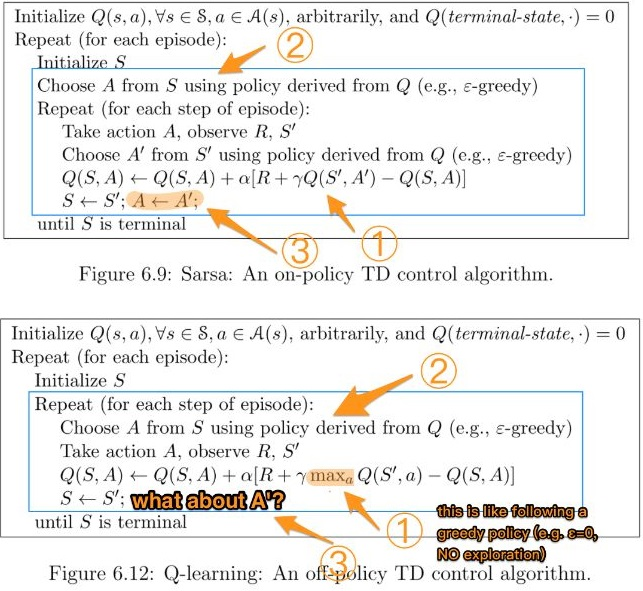
\includegraphics[scale=0.7]{pix/sarsa.jpg}
\caption{SARSA: An on-policy TD control algorithm}
\label{fig:SARSA}
\end{figure}

\noindent Blue boxes highlight the part where the two algorithms actually differ. 
Numbers highlight the more detailed difference to be explained later.

\begin{table}[htb]   
\begin{center}   
%\caption{title}  
%\label{table:1} 
\begin{tabular}{|c|c|c|}   
\hline    & \textbf{SARSA} & \textbf{Q-learning} \\   
\hline   Choosing $A'$ & $\pi$ & $\pi$  \\ 
\hline   Updating $Q$ & $\pi$ & $\mu$  \\  
\hline   
\end{tabular}   
\end{center}   
\end{table}

\noindent where $\pi$ is a $\epsilon$-greedy policy (e.g. $\epsilon > 0$ with 
exploration), and $\mu$ is a greedy policy (e.g. $\epsilon \equiv 0$, 
NO exploration).
\begin{itemize}
%\setlength{\itemsep}{0pt}
%\setlength{\parsep}{0pt}
\setlength{\parskip}{0pt}
\item[1.]
Given that $Q$-learning is using different policies for choosing next 
action $A'$ and updating $Q$. In other words, it is trying to evaluate 
$\pi$ while following another policy $\mu$, so it's an off-policy algorithm.
\item[2.]
In contrast, SARSA uses $\pi$ all the time, hence it is an on-policy algorithm.
\end{itemize}

\noindent {\bf More detailed explanation:}
\begin{itemize}
%\setlength{\itemsep}{0pt}
%\setlength{\parsep}{0pt}
\setlength{\parskip}{0pt}
\item[1.]
The most important difference between the two is how $Q$ is updated after 
each action. SARSA uses the $Q'$ following a $\epsilon$-greedy policy 
exactly, as $A'$ is drawn from it. In contrast, $Q$-learning uses the 
maximum $Q'$ over all possible actions for the next step. This makes it look 
like following a greedy policy with $\epsilon \equiv 0$, i.e. NO exploration 
in this part.
\item[2.]
However, when actually taking an action, $Q$-learning still uses the action 
taken from a $\epsilon$-greedy policy. This is why "Choose A ..." is inside 
the repeat loop.
\item[3.]
Following the loop logic in $Q$-learning, $A'$ is still from the 
$\epsilon$-greedy policy.
\end{itemize}

Congratulations for the beautiful graphics and pics. Years after I asked 
this question I came to realise that the state and action iteration, and 
the policy value iteration and update, are two different processes. Sadly, 
Sutton and Barto don't make this very clear. How you decide on actions 
affects the algorithms as you explained. Max action in $Q$-Learning usually 
implies choosing the action with next best $Q(s,a)$ e.g., greedy. In Sarsa 
this isn't the case, you either follow the policy (on-line) or you explore 
a new one depending on a random probability. Your description is spot on!

\subsubsection{Answers from Partagons and others(知乎)}

比如说现在有某个策略$\pi$,根据这个策略走到状态$s'$时应该采取动作$a'$。
\begin{itemize}
%\setlength{\itemsep}{0pt}
%\setlength{\parsep}{0pt}
\setlength{\parskip}{0pt}
\item[1)]
Sarsa更新$Q$值的方式是:
$$
Q(s,a) \leftarrow Q(s,a) + \alpha (R + \gamma Q(s',a') - Q(s,a))
$$
\noindent 更新值的时候是依据$a'$,也就是说确实采用了既有的策略$\pi$,所以叫on-policy

\item[2)]
$Q$-learning更新$Q$值的方式是:
$$
Q(s,a) \leftarrow Q(s,a) + \alpha (R + \gamma \max_aQ(s',a) - Q(s,a))
$$
\noindent 这里更新的时候没有用到$a'$啊,而是直接取了使$Q$值最大的那个动作$a$,
和既有的策略$\pi$是不一样的,所以叫off-policy
\end{itemize}

\begin{emp_box}
\indent 把on-policy翻译为同策略,off-policy翻译为异策略,比较好理解,指的是用来评价改进
的目标策略(target policy)与{\bf 学习过程中}做决策产生样本的行为策略(behavior 
policy)的异同。
\end{emp_box}




%+++++++++++++++++++++++++++++++++++++++++++
% 2.4 Why using behavior policy instead of target policy
%-------------------------------------------
\section{Why using behavior policy instead of target policy}

why to use different policy in order to build the action value 
function?

\begin{emp_box}
An advantage of this separation is that the target policy may 
be deterministic (e.g., greedy), while the behavior policy can 
continue to sample all possible actions.
\end{emp_box}

The more usual way of framing it is exploration vs 
exploitation. Theory tells you in standard MDPs that the 
optimal policy will be deterministic - each state has one 
"best" action that you should always take for optimal 
behaviour (sometimes more than one equivalent action, but 
in that circumstance you can always choose which one 
deterministically).

So you end up with some difficult issues using an on-policy 
control approach:
\begin{itemize}

\item
If you work with a single deterministic policy as your 
behaviour policy during learning, you will not learn enough 
about alternative behaviours in order to find better outcomes 
and improve the policy.

\item
If you work with a stochastic policy that covers all 
possible choices - to guarantee exploration - you know that 
can never be optimal. Careful manipulation of how the 
stochastic part varies (such as reducing $\epsilon$ in 
$\epsilon$-greedy policies) can get you arbitrarily close 
to a truly optimal policy, but then you are using the same 
parameters to manipulate both exploration rate and closeness 
to optimality of your learned policy, which means 
compromising between best exploration and the best end results.
\end{itemize}

\begin{emp_box}
What it makes it more interesting than an on policy method 
that only use a single policy?
\end{emp_box}


With off-policy learning, a target policy can be your best 
guess at deterministic optimal policy. Whilst your behaviour 
policy can be chosen based mainly on exploration vs 
exploitation issues, ignoring to some degree how the 
exploration rate affects how close to optimal the behaviour 
can get.

It is worth noting that some environments can be simple 
enough or stochastic enough with state transition and reward, 
that you can use a deterministic policy with and on-policy 
learner to explore and learn optimal control. However, you 
cannot rely on that in general, it would be more common that 
such an agent would stop learning at some point, far short 
of being optimal.


%+++++++++++++++++++++++++++++++++++++++++++
% 2.5 An example
%-------------------------------------------
\section{An example}

\begin{figure}[ht]
\centering
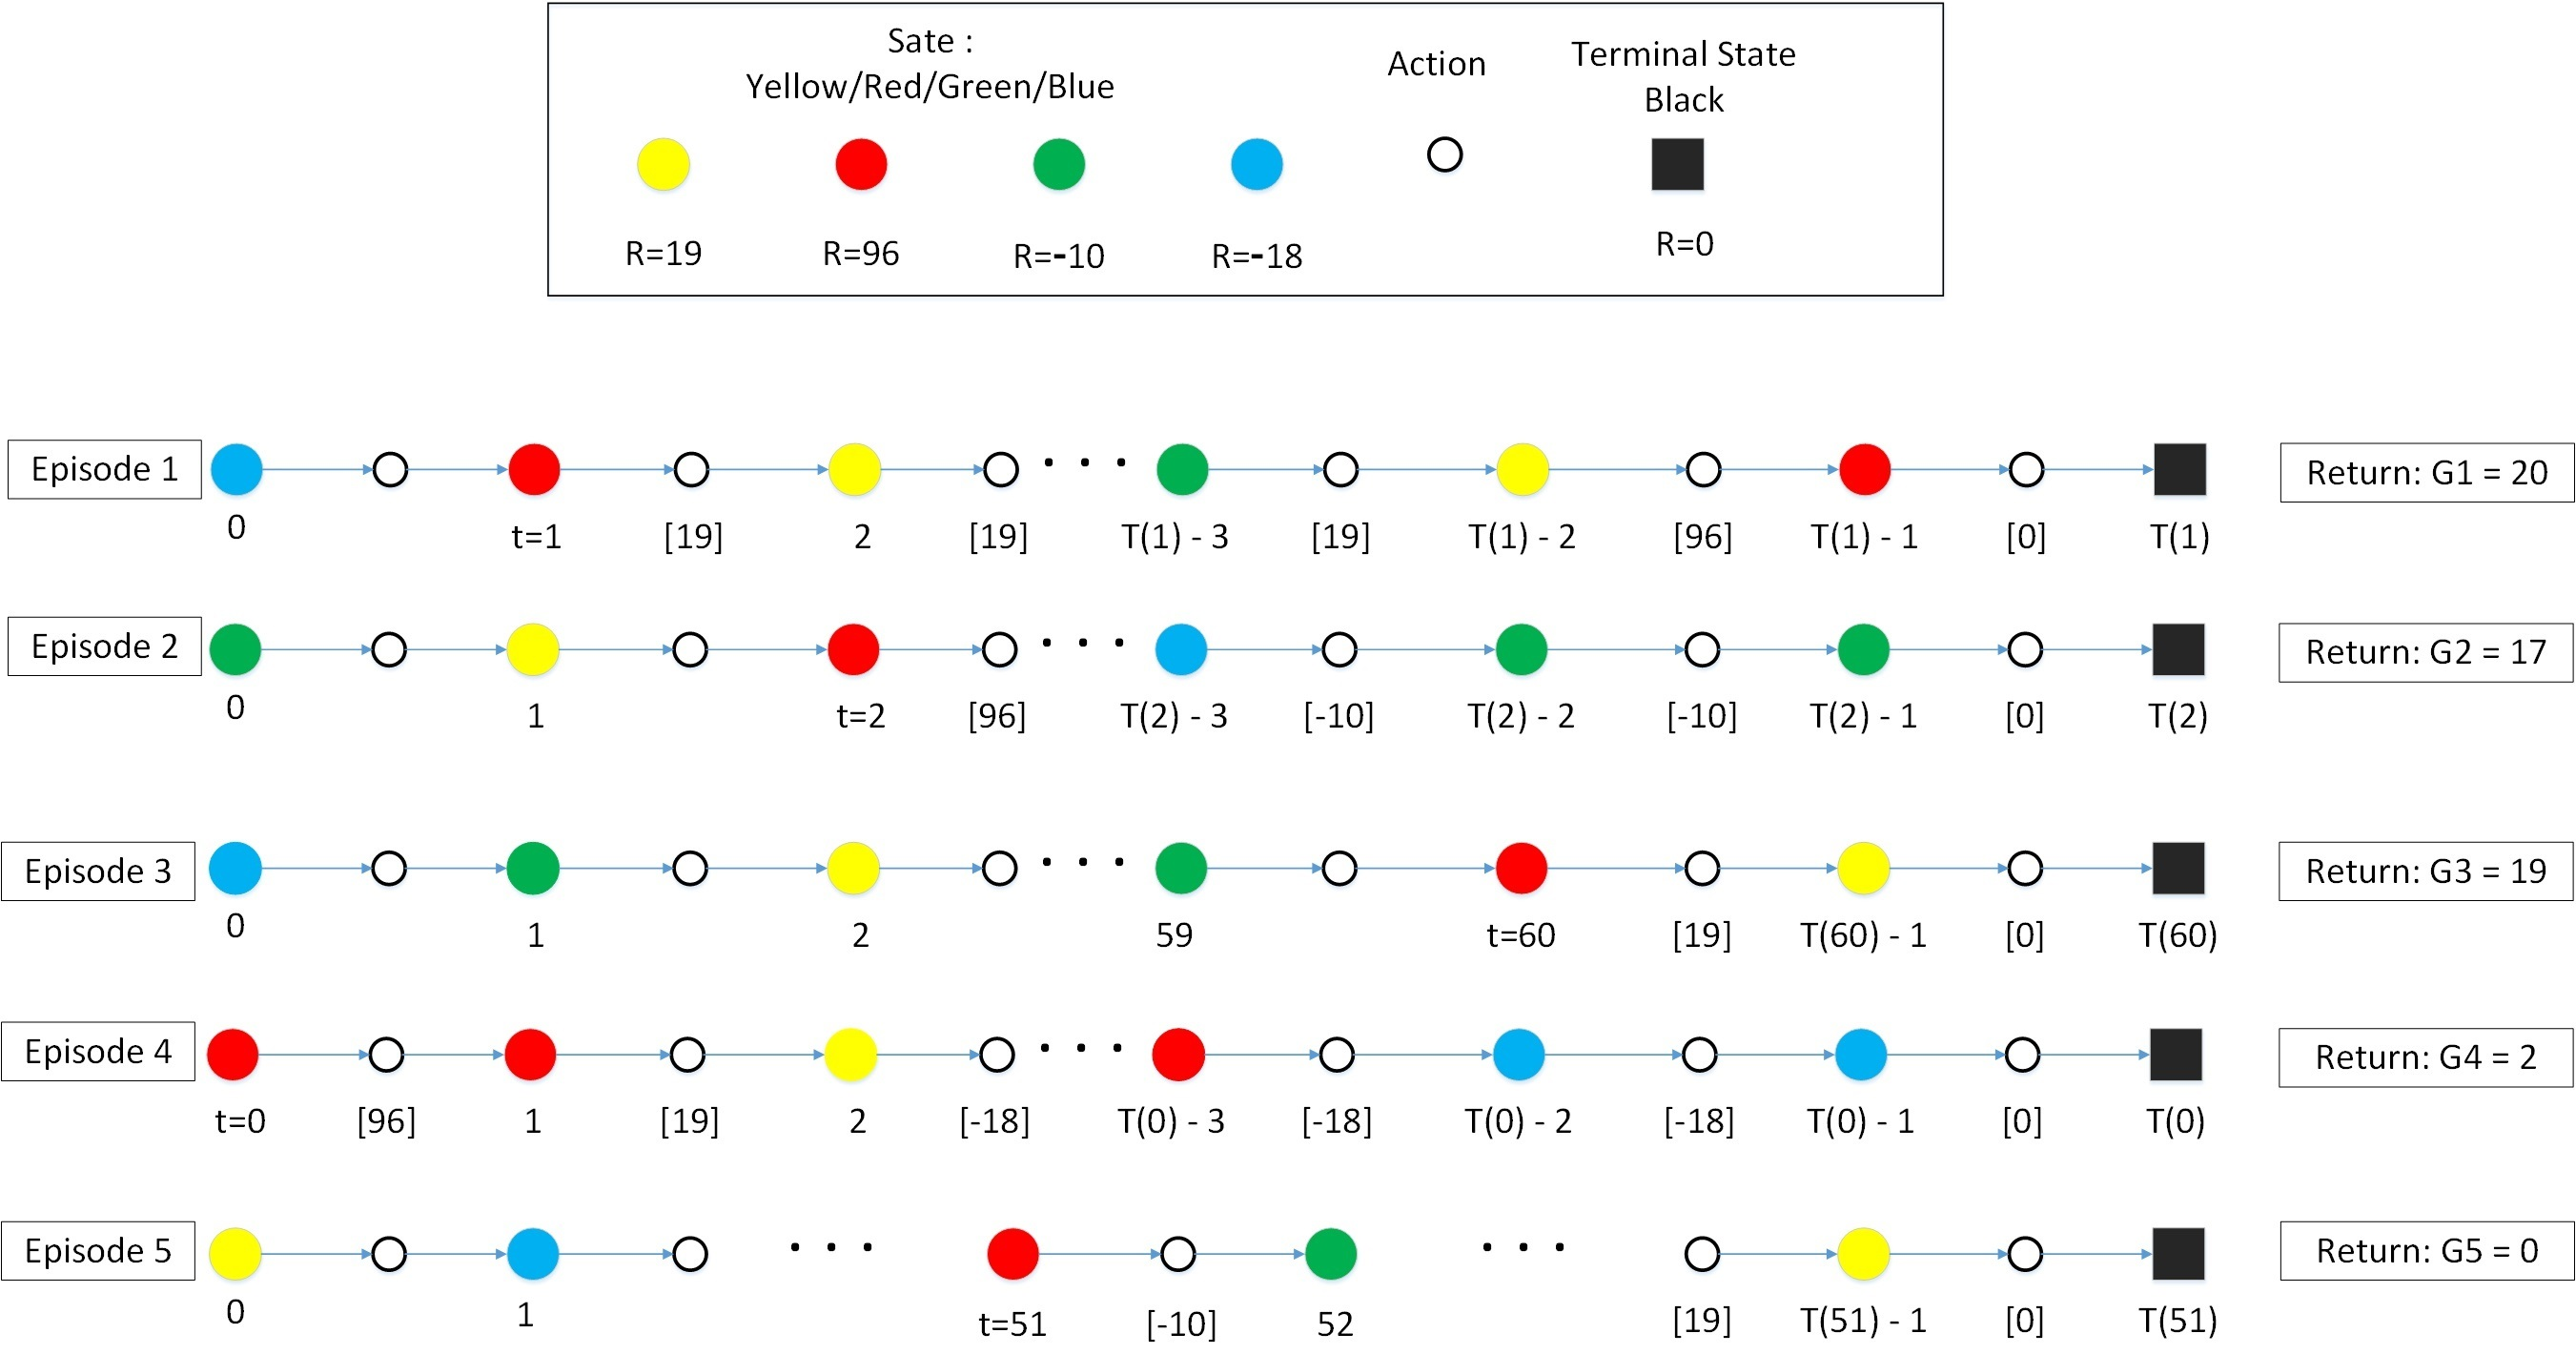
\includegraphics[scale=0.17]{pix/example.jpg}
\caption{An Example of Monte Carlo Methods with First-visit Technic}
%\label{fig:label}
\end{figure}

本例子基于Monte Carlo过程,环境的动态情况未知(即状态转移概率未知)。并采用
first-visit方法,即指定计算某一个状态(State)的价值时,只计算每个回合第一次出现
该状态(State)之后到结束的总奖励(Return)。

有五个状态:黄、红、绿、蓝、黑。其中黑状态为终止状态(Terminal)。在第一个框中每个
状态下面为即时奖励(Reward)。在此为了简化例子不具体列出动作,用一个空心环代替动作
集合的任一动作。当遇到黑色时就结束当前回合(Episode)。我们用$t$表示第一次遇到指定
状态的时间步,在本例中指定计算红色状态的价值(Red State Value),$T(t)$
表示一个回合中的终点的时间步。

\subsubsection{1. 采样}

基于行为策略$b$与环境互动,经过采样后,我们得到五个回合(省略部分为动作-状态序列)。

\subsubsection{2.计算每个样本回合的Return}

在这里取第三个回合(Episode 3)分析,假设在其省略序列部分没有出现红色,第一次遇到红色在
第60时间步(Time Step),则从此时开始计算后面的奖励。第61步为黄色,可得奖励19,第62步
为黑色,可得奖励0,并终止回合。经计算后该回合从第一个红色状态开始后得到的总奖励G3
(Return)为19。

其他回合也是这样处理算出每个回合的Return。(假设其他回合的省略部分随机出现除了黑色以外
的所有状态)

\subsubsection{3.计算行为策略b的红色状态的价值期望}

由Monte Carlo计算方法可知
$$
v_b(S_t=\text{Red})=E[G_t|S_t=\text{Red}]
=(G_1+G_2+G_3+G_4+G_5)/5 = 11.6
$$

11.6为在行为策略$b$下时,红色状态的价值(即Return的期望值)。在实际应用中,根据大数定理,
采样回合(Episode)的数量一般需要成千上万个,才能保证所计算的结果接近期望值。
On-policy中就是应用这个价值来进行学习、改善策略的,也即基于贪婪思想选取最大值的动作,
然后作为新的On-policy的策略。

\subsubsection{4. 计算目标策略$\pi$的红色状态的价值期望}

由于importance-sampling ratio 均可由公式\eqref{sate_gain_expectation}计算得到,所以这里未给出具体的动作及其在
相应策略下的概率以简化问题,因此在这里假设$\rho_1^{T(1)-1}$、$\rho_2^{T(2)-1}$、
$\rho_60^{T(60)-1}$、$\rho_0^{T(0)-1}$、$\rho_51^{T(51)-1}$分别为5,10,5,20,10。
有以下运算:
\begin{align*}
&\quad\ v_t(S_t=\text{Red}) \\
&= E[\rho_t^{T-1}G_t|S_t=\text{Red}] \\
&= (\rho_1^{T(1)-1}G_1 + \rho_2^{T(2)-1}G_2 + 
\rho_60^{T(60)-1}G_3 + \rho_0^{T(0)-1}G_4 + \rho_51^{T(51)-1}G_5)/5 \\
&= (5*20 + 10*17 +5*19 + 20*2 + 10*0) / 5 \\
&= 81
\end{align}

因此81为我们从由行为策略$b$产生的五个Episode中,所得到的目标策略$\pi$下的红色状态的价值
(即目标策略下的红色状态的Returne期望值)。然后根据该价值来学习,也即基于贪婪思想选取最大
值的动作,然后作为新的目标策略$\pi$。 

上述方法可称为普通的重要度采样,与之对应的还有加权重要度采样(本文不赘述,可在Sutton书中的
第五章查看)。前者在统计学意义上是无偏估计,但方差很大(比如在上述例子中11.6与81),后者则
是有偏估计(偏差逐渐收敛到0),方差也能收敛到零。

On-policy-与Off-policy的区别在于:更新价值所使用的方法是沿着既定的策略(on-policy)抑
或是新策略(off-policy)。

\cite{Sutton1998}
%\parencite{Sutton1998}

